%%%%%%%%%%%%%%%%%%%%%%%%%%%%%%%%%%%%%%%%%
% Beamer Presentation
% LaTeX Template
% Version 1.0 (10/11/12)
%
% This template has been downloaded from:
% http://www.LaTeXTemplates.com
%
% License:
% CC BY-NC-SA 3.0 (http://creativecommons.org/licenses/by-nc-sa/3.0/)
%
%%%%%%%%%%%%%%%%%%%%%%%%%%%%%%%%%%%%%%%%%

%----------------------------------------------------------------------------------------
%	PACKAGES AND THEMES
%----------------------------------------------------------------------------------------

\documentclass{beamer}

\mode<presentation> {

% The Beamer class comes with a number of default slide themes
% which change the colors and layouts of slides. Below this is a list
% of all the themes, uncomment each in turn to see what they look like.

%\usetheme{default}
%\usetheme{AnnArbor}
%\usetheme{Antibes}
%\usetheme{Bergen}
%\usetheme{Berkeley}
%\usetheme{Berlin}
%\usetheme{Boadilla}
\usetheme{CambridgeUS}
%\usetheme{Copenhagen}
%\usetheme{Darmstadt}
%\usetheme{Dresden}
%\usetheme{Frankfurt}
%\usetheme{Goettingen}
%\usetheme{Hannover}
%\usetheme{Ilmenau}
%\usetheme{JuanLesPins}
%\usetheme{Luebeck}
%\usetheme{Madrid}
%\usetheme{Malmoe}
%\usetheme{Marburg}
%\usetheme{Montpellier}
%\usetheme{PaloAlto}
%\usetheme{Pittsburgh}
%\usetheme{Rochester}
%\usetheme{Singapore}
%\usetheme{Szeged}
%\usetheme{Warsaw}

% As well as themes, the Beamer class has a number of color themes
% for any slide theme. Uncomment each of these in turn to see how it
% changes the colors of your current slide theme.

%\usecolortheme{albatross}
%\usecolortheme{beaver}
%\usecolortheme{beetle}
%\usecolortheme{crane}
%\usecolortheme{dolphin}
%\usecolortheme{dove}
%\usecolortheme{fly}
%\usecolortheme{lily}
%\usecolortheme{orchid}
%\usecolortheme{rose}
%\usecolortheme{seagull}
%\usecolortheme{seahorse}
%\usecolortheme{whale}
%\usecolortheme{wolverine}

%\setbeamertemplate{footline} % To remove the footer line in all slides uncomment this line
%\setbeamertemplate{footline}[page number] % To replace the footer line in all slides with a simple slide count uncomment this line

%\setbeamertemplate{navigation symbols}{} % To remove the navigation symbols from the bottom of all slides uncomment this line
}

\usepackage{graphicx} % Allows including images
\usepackage{booktabs} % Allows the use of \toprule, \midrule and \bottomrule in tables


%----------------------------------------------------------------------------------------
%	TITLE PAGE
%----------------------------------------------------------------------------------------

\title[Classification of SPD matrices]{Classification of SPD matrices using a Riemannian-based kernel} % The short title appears at the bottom of every slide, the full title is only on the title page

\author{Anna Kuzina} % Your name
\institute[Skoltech, HSE] % Your institution as it will appear on the bottom of every slide, may be shorthand to save space
{
Skoltech, HSE \\ % Your institution for the title page
\medskip
\textit{anna.kuzina@skoltech.ru} % Your email address
}
\date{\today} % Date, can be changed to a custom date

\begin{document}

\begin{frame}
\titlepage % Print the title page as the first slide
\end{frame}

%\begin{frame}
%\frametitle{Overview} % Table of contents slide, comment this block out to remove it
%\tableofcontents 
%\end{frame}

%----------------------------------------------------------------------------------------
%	PRESENTATION SLIDES
%----------------------------------------------------------------------------------------


%\begin{frame}
%\frametitle{Motivation}
%\textbf{Problem:} Detection of depression and epilepsy from fMRI data
%\vfill
%\begin{itemize}
%	\item Depression --- the most prevalent psychiatric illnesses. 
%		\vfill
%	\item It causes deviations in the structure and functioning of neuronal brain networks 
%		\vfill
%	\item More than one third of people with epilepsy suffer from depression 
%		\vfill
%	\item There are no \textbf{biological} tests for depression diagnosis
%\end{itemize}
%
%\end{frame}

%------------------------------------------------


\begin{frame}
\frametitle{Motivation}

\uncover<1->{
	\textbf{Where do SPD matrices come from?}}
\begin{itemize}
	\item<1-> fMRI (functional magnetic resonance imaging) enables us to build a graph, representing connections of different parts of the brain
	\vfill
	\item<1-> 	Structural connectome can be seen as a symmetric adjacency matrix
	\vfill 
	\item<1-> We want to take into account geometry of the data
	
\end{itemize}

\end{frame}

%------------------------------------------------


\begin{frame}
\frametitle{From SI to SPD}
\begin{enumerate}
	\item Laplacian of the SI adjacency matrix  --- SPSD matrix
	\begin{equation*}
	L_S = D_S - S
	\end{equation*}
	\vfill
%	\uncover<2->{
		\item Add regularization
		\begin{equation*}
		P  = L_{S} + \lambda I, \; \lambda > 0
		\end{equation*}
	%}
\end{enumerate}

\end{frame}

%------------------------------------------------


\begin{frame}
\frametitle{Basic notations}
\begin{itemize}
	\item $\mathcal{M}(n)$ --- space of $n\times n$ real matrices
	\vfill
	\item $\{S \in \mathcal{M}(n): S^T = S  \}$ --- space of $n\times n$ symmetric matrices
		\vfill
	\item $\{P \in S(n): u^TPu > 0 \; \forall u \in \mathbb{R}^n  \}$ --- space of $n\times n$ SPD matrices
		\vfill
	\item $\exp(S) = C\; \text{diag}(\exp(\lambda_1), \dots, \exp(\lambda_n) ) \; C^T  \in P(n)$
		\vfill
	\item $\log(P) = C\; \text{diag}(\log(\lambda_1), \dots, \log(\lambda_n) ) \; C^T \in S(n)$
		\vfill
	\item $P^{\frac12}$ --- symmetric matrix $A$, s.t. $AA = P$
\end{itemize}

\end{frame}

%------------------------------------------------

\begin{frame}
\frametitle{Riemannian manifold}
\begin{itemize}
\item Smooth manifold
\item Tangent finite-dimensional Euclidean space at every point with inner product $g_P$
\item $g_P$, Riemannian metric, varies smoothly from point to point
\end{itemize}
 \hfill 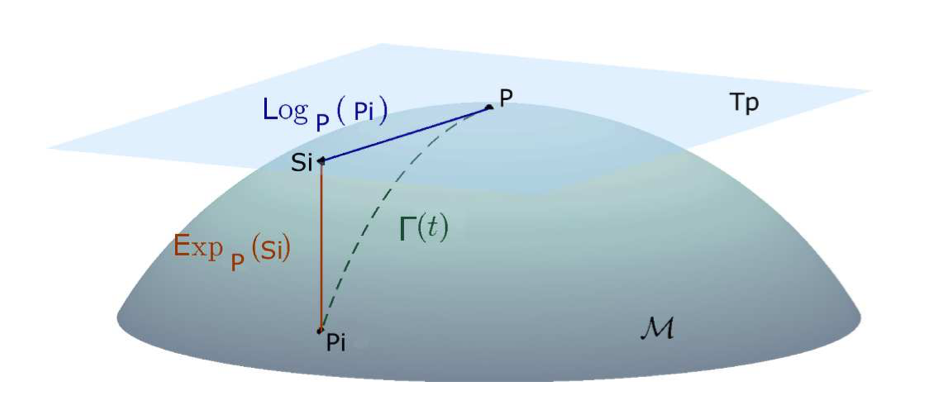
\includegraphics[scale=0.5]{manifold.png}
\end{frame}


%------------------------------------------------

\begin{frame}
\frametitle{Affine-invariant metrics}
Scalar product on the Tangent space at identity generates metrics on the whole Lie group. 
\begin{block}{Dot product at Identity}
	\begin{equation*}
	\langle S_1, S_2 \rangle_I = \text{Tr}(S_1 S_2^T) = \text{Tr}(S_1 S_2), \quad S_1, S_1 \in T_I \mathcal{M}
	\end{equation*}
\end{block}

\begin{block}{Action of Linear group on a Lie group, Pennec et al. 2006}
	\begin{equation*}
	 A \odot P = A P A^T, \; A\in GL(n)
	\end{equation*}
\end{block}

\begin{block}{Invariance under congruent transformations, Novikov and Taymanov 2005}
	\begin{equation*}
	\forall g \in T_P \quad 
	 \langle S_1, S_2 \rangle_P =  \langle g \odot S_1,g\odot  S_2 \rangle_{g \odot P}
	%= \text{Tr}(S_1 P^{-1}S_2 P^{-1})
	\end{equation*}
%	\begin{equation*}
%	\forall h \in T_P \quad 
%	\langle S_1h, S_2h \rangle_P = \langle S_1, S_2 \rangle_P =  \langle S_1P^{-1}, S_2P^{-1} \rangle_I
%	\end{equation*}
\end{block}

\begin{block}{Affine-invariant metric}
	\begin{equation*}
	\langle S_1, S_2 \rangle_P = \text{Tr}(S_1 P^{-1}S_2 P^{-1}) = \text{Tr}(P^{-1}S_1 P^{-1}S_2)
	\end{equation*}
\end{block}
\end{frame}

%------------------------------------------------

\begin{frame}
\frametitle{Riemannian metrics}
\begin{block}{Induced Norm}
	\begin{equation*}
	\|S \|_P^2 = 	\langle S, S \rangle_P  = \text{Tr}((S P^{-1})^2)
	\end{equation*}
\end{block}

$P = I:$
\begin{equation*}
\|S\|_I^2 = \text{Tr}(S^2) =  \text{Tr}(S^TS) = \|S\|_F^2 = \|\text{vect}(S)\|_2^2
\end{equation*}
\begin{equation*}
\text{vect}(S) = \left[ S_{1,1}, \sqrt{2}S_{1,2}, S_{2,2}, \sqrt{2}S_{1,3} ,  \sqrt{2}S_{2,3}, S_{3,3}, \dots, S_{n,n}  \right]^T
\end{equation*}

\end{frame}
%------------------------------------------------

\begin{frame}
\frametitle{Riemannian Geodesic distance}

\begin{block}{}
	The geodesic --- shortest path between two points\\
	Riemannian distance --- length of the geodesic
\end{block}
	\uncover<2->{
\begin{block}{}
		\begin{equation*}
	\Gamma(t): [0,1] \rightarrow P(n)
	\end{equation*}
	Norm of the tangent vector --- instantaneous speed of the geodesic 
	\begin{equation*}
	L(\Gamma(t)) = \int_{0}^{1} \|\dot{\Gamma(t)}\|_{\Gamma(t)}dt
	\end{equation*}
\end{block}}
%\begin{columns}[c] 
%	\uncover<2->{
%\column{.45\textwidth} % Left column and width
% $S_i$ can be seen as derivative of the geodesic between $P$ and $P_i$ at point $t=1$}
%\column{.5\textwidth} % Right column and width
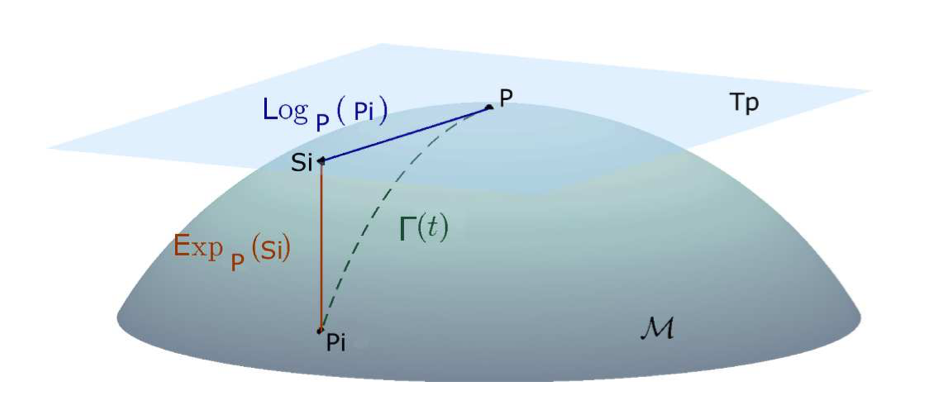
\includegraphics[scale=0.45]{manifold.png}
%\end{columns}

\end{frame}

%------------------------------------------------

\begin{frame}
\frametitle{Geodesic}
For the invariant metric, geodesic is generated by the action of one-parameter subgroup (Sternberg 1964)

\begin{block}{One-parameter subgroup}
	\begin{equation*}
	x = \exp(tS)
	\end{equation*}
\end{block}

\begin{block}{Geodesic going through $I$ with tangent vector $S$}
	\begin{equation*}
		\Gamma_{I,S}(t) = \exp(tS)^{\frac12}I\exp(tS)^{\frac12} = \exp({tS})
	\end{equation*}
\end{block}
\end{frame}

%------------------------------------------------

\begin{frame}
\frametitle{Geodesic}

\begin{block}{Geodesic, starting from identity}
	\begin{align*}
			\Gamma_{I,S}(t) &= \exp(tS)
	\end{align*}
\end{block}

\begin{block}{ }
	Using invariance
	\begin{equation*}
	A \odot \Gamma_{P,S}(t) = \Gamma_{A \odot P ,A \odot S }(t) , \quad A = P^{-\frac12}
	\end{equation*}
	
	\begin{equation*}
	 \Gamma_{P,S}(t) = P^{\frac12} \Gamma_{I,A^{-\frac12}SA^{-\frac12}}(t) P^{\frac12}  = 
	  P^{\frac12} \exp( t P^{-\frac12}SP^{-\frac12} )P^{\frac12} 
	\end{equation*}
\end{block}
\end{frame}

%------------------------------------------------

\begin{frame}
\frametitle{Exponential map}
\begin{block}{Exponential mapping (from tangent space to the manifold)}
	\begin{equation*}
	\exp_P(S_i)  = P_i = P^{\frac12} \exp(P^{-\frac12}S_iP^{-\frac12})P^{\frac12}
	\end{equation*}
\end{block}
\vfill
\begin{block}{Logarithmic mapping (from the manifold on the tangent space)}
	\begin{equation*}
	\log_P(P_i)  = S_i = P^{\frac12} \log(P^{-\frac12}P_iP^{-\frac12})P^{\frac12}
	\end{equation*}
\end{block}
\end{frame}
%------------------------------------------------
\begin{frame}
\frametitle{Riemannian distance}
\begin{block}{ }
	\begin{align*}
	L(\Gamma(t)) & = \int_{0}^{1} \|\dot{\Gamma(t)}\|_{\Gamma(t)}dt =  \int_{0}^{1}\sqrt{\langle \dot{\Gamma(t)}, \dot{\Gamma(t)} \rangle_{\Gamma(t)}}dt = \\
	 & =   \int_{0}^{1}\sqrt{Tr\left( (\dot{\Gamma(t)}\Gamma(t)^{-1})^2 \right) }dt
	\end{align*}
\end{block}
Again we start from the identity.

Having $S =  C\text{diag}(\lambda_i)C^T$, where $C$ is a unitary matrix:
\begin{block}{ }
	\begin{align*}
	&\dot{\Gamma}_{I,S}(t) = C\text{diag}(\lambda_i\exp(t \lambda_i))C^T \\
	&\Gamma_{I,S}(t)^{-1} = C\text{diag}(\exp( - t \lambda_i))C^T \\
&	\dot{\Gamma}_{I,S}(t)\Gamma_{I,S}(t)^{-1} = C\text{diag}(\lambda_i\exp(t \lambda_i))\text{diag}(\exp( - t \lambda_i))C^T = \\&=C\text{diag}(\lambda_i) C^T = S
	\end{align*}
\end{block}

\end{frame}

%------------------------------------------------
\begin{frame}
\frametitle{Riemannian distance}

\begin{block}{ }
	\begin{align*}
	L(\Gamma(t)) = \int_{0}^{1}\sqrt{Tr\left( (\dot{\Gamma(t)}\Gamma(t)^{-1})^2 \right) }dt
	\end{align*}
\end{block}

\begin{block}{Distance to the Identity}
	\begin{align*}
	\sigma_R (I, P) =L(\Gamma_{I,S}(t)) = \int_{0}^{1}\sqrt{Tr\left( S^2 \right) }dt = \|S\|_F = \|\log(P)\|_F
	\end{align*}
\end{block}

\begin{block}{Affine invariance}
	\begin{align*}
	\sigma_R (P_1, P_2) & = \sigma_R(A \odot P_1, A \odot P_1), \quad A = P_1^{-\frac12} \\
 \sigma_R (P_1, P_2) & =  \sigma_R (I , P_1^{-\frac12}P_2P_1^{-\frac12})	= \|\log(P_1^{-1}P_2)\|_F = \left( \sum \log^2\lambda_i \right)^{\frac12}
	\end{align*}
\end{block}
\end{frame}



%------------------------------------------------

\begin{frame}
\frametitle{ Classification in the Riemannian manifold}
\begin{itemize}
	\item Minimum distance to Riemanian Mean
\begin{block}{Geometric mean}
	\begin{equation*}
	P^* = \arg\min_P \sum_{i=1}^{m}\sigma^2_R(P, P_i)
	\end{equation*}
\end{block}
\vfill
\item kNN with Riemannian distances
\end{itemize}

\end{frame}

%------------------------------------------------



\begin{frame}
\frametitle{Kernel Approach}

\begin{block}{Mapping function}
	\begin{equation*}
		\phi (P_i) = \log_{P^*}(P_i)
	\end{equation*}
\end{block}
\begin{block}{Riemannian base kernel}
	\begin{equation*}
 k_R(P_i,P_j) = \langle 	\phi (P_i), 	\phi (P_j)\rangle_{P^*} = \text{Tr}( \log_{P^*}(P_i)P^{*-1} \log_{P^*}(P_j)P^{*-1}) = 
	\end{equation*}
	\begin{equation*}
 =	\text{Tr}( \log (P^{*-\frac12}P_i P^{*-\frac12}) \log (P^{*-\frac12}P_j P^{*-\frac12})) =	\text{Tr}(\tilde{P_i}\tilde{P_j}) = 
	\end{equation*}
	\begin{equation*}
	= \langle \tilde{P_i},\tilde{P_j} \rangle_F =  \text{vect}(\tilde{P_i})^T  \text{vect}(\tilde{P_j}) =  \langle  \text{vect}(\tilde{P_i}), \text{vect}(\tilde{P_j}) \rangle_2
	\end{equation*}
\end{block}

\end{frame}

%------------------------------------------------


\begin{frame}
\frametitle{Reference point}
	\begin{equation*}
k_R(P_i,P_j) = \text{Tr}( \log (P^{*-\frac12}P_i P^{*-\frac12}) \log (P^{*-\frac12}P_j P^{*-\frac12})) =	\text{Tr}(\tilde{P_i}\tilde{P_j})
\end{equation*}
\uncover<2->{
\begin{block}{log-Euclidean kernel}
	$$
	P^* = I
	$$
\begin{equation*}
  k_{LE}(P_i,P_j)  = \text{Tr}(\log(P_i)\log(P_j))
\end{equation*}
\end{block}}
\uncover<3->{
\begin{block}{Geometric mean}
\begin{equation*}
	P^* = \arg\min_P \sum_{i=1}^{m}\sigma^2_R(P, P_i)
\end{equation*}	
\end{block}}

\end{frame}

%------------------------------------------------

%
%\begin{frame}
%\frametitle{Results}
%\begin{table}[!h]
%	\caption{ROC-AUC of the best model}
%	\begin{center}
%		\begin{tabular}{| c | c | c | c|}
%			\hline
%%			\multicolumn{4}{ c |}{\textbf{kNN parameters}}  & \textbf{Equipo} \\ 
%%			\cline{1-4}
%			Problem & Riemannian Kernel & Euclidean Kernel  & Graph features\\ \hline
%			E vs C  & 0.69&0.69  &\textbf{0.76}  \\
%			D vs C &  \textbf{0.70} &  0.58 &0.61 \\ 
%			DE vs E & \textbf{0.77} & \textbf{0.77}  &0.66 \\
%			DE vs D & \textbf{0.70} &  0.66 &0.66\\
%			\hline
%		\end{tabular}
%	\end{center}
%\end{table}
%
%\begin{table}[!h]
%	\caption{Accuracy}
%	\begin{center}
%		\begin{tabular}{| c | c | c | }
%			\hline
%			%			\multicolumn{4}{ c |}{\textbf{kNN parameters}}  & \textbf{Equipo} \\ 
%			%			\cline{1-4}
%			Problem & Riemannian Kernel & Euclidean Kernel  \\ \hline
%			E no E &\textbf{0.58 }&0.55\\
%			D no D & 0.68 & 0.68  \\
%			E vs C  & \textbf{0.59} & 0.58   \\
%			D vs C &\textbf{0.67}&  0.58  \\ 
%			DE vs E & 0.70 & 0.70 \\
%			DE vs D &\textbf{0.73 }&  0.69 \\
%			\hline
%		\end{tabular}
%	\end{center}
%\end{table}
%
%D --- patients with depression\\
%E --- patients with epilepsy\\ 
%C --- healthy people\\
%DE --- patients with both depression and epilepsy\\
%
%
%\end{frame}

%------------------------------------------------

%\begin{frame}
%\frametitle{Results}
%\begin{table}[!h]
%	\caption{False negative rate (for FP = 0.3)}
%	\begin{center}
%		\begin{tabular}{| c | c | c | c|}
%			\hline
%			Problem & Riemannian Kernel & Euclidean Kernel  \\ \hline
%			E no E &\textbf{0.44} &0.74\\
%			D no D & 0.36 & 0.36  \\
%			E vs C  & 0.32&0.32   \\
%			D vs C &  \textbf{0.36} &  0.72  \\ 
%			DE vs E & 0.36 & 0.36   \\
%			DE vs D & \textbf{0.36} &  0.40 \\
%			\hline
%		\end{tabular}
%	\end{center}
%\end{table}
%
%D --- patients with depression\\
%E --- patients with epilepsy\\ 
%C --- healthy people\\
%DE --- patients with both depression and epilepsy\\
%
%
%\end{frame}


\begin{frame}
\frametitle{Riemannian Network}
\begin{block}{BiMap Layer}
	\begin{equation*}
		X_k = W_k X_{k-1}W_k^T
	\end{equation*}
	$W_k$ --- row full-rank matrix
\end{block}

\begin{block}{ReEig Layer}
	\begin{equation*}
	X_k = U_{k-1} \max (\varepsilon I, \Sigma_{k-1})U_{k-1}^T
	\end{equation*}
	$X_{k-1} = U_{k-1}\Sigma_{k-1} U_{k-1}^T$
\end{block}

\begin{block}{LogEig Layer}
	Projection on the tangent plane at Identity
	\begin{equation*}
	X_k = U_{k-1} \log ( \Sigma_{k-1})U_{k-1}^T
	\end{equation*}
\end{block}

\end{frame}

%------------------------------------------------
%------------------------------------------------
\begin{frame}
\frametitle{References}
\footnotesize
\begin{thebibliography}{99} % Beamer does not support BibTeX so references must be inserted manually as below
\bibitem[Smith, 2012]{p1} M. Moakher (2005)
\newblock Symmetric Positive-Definite Matrices: From Geometry to Applications and Visualization
	
\bibitem[]{p1}X. Pennec et al. (2006)
\newblock A Riemannian Framework For Tensor Computing 
	
%\bibitem[Smith, 2012]{p1} A. Barachant et al. (2010)
%\newblock Riemannian Geometry Applied to BCI Classification

\bibitem[Smith, 2012]{p2} A. Barachant et al.(2012)
\newblock Multiclass Brain-Computer Interface Classification by Riemannian Geometry

\bibitem[qq]{p4}  A. Pimkin, M. Belyaev et al. (2017)
\newblock Classification of brain network structures using analysis of symmetric semidefinite matrices

\bibitem[qq]{p4}  S. Novikov, I. Taymanov. (2005)
\newblock Modern geometric structures and fields

\bibitem[qq]{p4}  S. Stenberg (1964)
\newblock Lectures in differential geometry
\end{thebibliography}
\end{frame}

%------------------------------------------------

\begin{frame}
\Huge{\centerline{The End}}
\end{frame}

%----------------------------------------------------------------------------------------

\end{document} 